%!TEX encoding = UTF-8 Unicode
% ================================================================================
\documentclass[
    fontsize=12pt,
    headings=small,
    parskip=half,           % Ersetzt manuelles Setzen von parskip/parindent.
    bibliography=totoc,
    numbers=noenddot,       % Entfernt den letzten Punkt der Kapitelnummern.
    open=any,               % Kapitel kann auf jeder Seite beginnen.
%   final                   % Entfernt alle todonotes und den Entwurfstempel.
    ]{scrreprt}
% ===================================Praeambel==================================
\include{stylesvs}
% ===================================Dokument===================================

\title{Entwicklung eines Visualisierungswerkzeuges zur Demons-
tration datenschutzfreundlicher Dokumentspeicherdienste}
\author{David Kirchhausen Monteiro}

\begin{document}

\begin{titlepage}% {{{
\includegraphics[width=6.8cm]{../pic/up-uhh-logo-u-2010-u-farbe-u-rgb.pdf}
\begin{center}\Large
	% Universität Hamburg \par
	% Fachbereich Informatik
	\vfill
	Bachelorarbeit
	\vfill
	\makeatletter
	{\Large\textsf{\textbf{\@title}}\par}
	\makeatother
	\vfill
	vorgelegt von
	\par\bigskip
	\makeatletter
	{\@author} \par
	\makeatother
	geb. am 24. Januar 1994 in Hildesheim \par
	Matrikelnummer 6530927 \par
	Studiengang Software-System-Entwicklung
	\vfill
	\makeatletter
	eingereicht am {\@date}
	\makeatother
	\vfill
	Betreuer: Maximilian Blochberger, M. Sc. \par
	Erstgutachter: Prof. Dr.-Ing. Hannes Federrath \par
	Zweitgutachter: Tilmann Stehle, M. Sc.
\end{center}
\ifoptionfinal{}{}
\end{titlepage}% }}}

\chapter*{Aufgabenstellung}

Im  Zuge  dieser  Bachelorarbeit  soll  ein  einfacher  Dokumentenspeicher  entwickelt  werden,
welcher möglichst viele Nutzerdaten erfasst und speichert. Die erfassten Daten sollen anschaulich
grafisch dargestellt werden können. Weiter sollen verschiedene Szenarien entwickelt werden,
welche aufzeigen wie eine mögliche Benutzung des Services mit und ohne der Verwendung
von datenschutzfreundlichen Methoden zum Anonymisieren von Daten aussieht. Anhand der
Szenarien soll eine grafische Auswertung Unterschiede zwischen anonymisierten Daten und
nicht anonymisierten Daten visuell sichtbar machen und die Unterschiede somit leicht zugänglich
sein.

\chapter*{Zusammenfassung}
\begin{enumerate}
\item Dokumentenspeicherdienste Vorteile (Problemstellung erläutern)
\item Mögliche Datenschutz unfreundliche Aspekte von gängigen Anbietern (Problemstellung erläutern)
\item Entwicklung des Dokumentenspeichers und der Visualisierung zur deutlich Veranschaulichung von Potentiellen Unterschieden zwischen der Verwendung von Datenschutz freundlichen Methoden zum Anonymisieren oder nicht. (Bearbeitung der Problemstellung)
\begin{enumerate}
\item Implementation des Dokumentenspeichers
\item Implementation der API zur Datenübergabe 
\item Implementation des Visualisierungswerkzeug
\item Darstellung der Szenarien zur Benutzung des Visualisierungswerkzeug
\end{enumerate}
\end{enumerate}

\tableofcontents

\chapter{Einleitung}

Dokumentenspeicherdienste sind nützliche Alltagsgegenstände, welche für private sowie kommerzielle Nutzer meist unverzichtbar sind. 
Sie bieten nicht nur den Speicherplatz für wichtige Dateien der Nutzer sondern stellen auch die Sicherheit der Dateien sicher und machen sie global jederzeit verfügbar. 
Durch die große Datensammlung dieser Dienstleister machen sie sich nicht nur selbst zu lukrativen Zielen von gezielten Angriffen (Yahoo, UBER etc.), jedoch auch die Dienstleister selber können die Daten auswerten und weitere Metadaten wie z.B. die Dateigröße oder den Autor der Datei sowie Verkehrsdaten wie z.B. die IP-Adresse oder die HTTP Header Felder über die Nutzer sammeln und weiterverwenden. 
Vor allem private Nutzer sind meist gar nicht über die Risiken und das Missbrauchspotenzial aufgeklärt, welche die Verwendung solcher Dienstleistungen mit sich bringen. 
Methoden zur Verschlüsselung oder das anonymisieren von Daten sind Benutzern meist nicht bekannt, werden von den Dienstanbietern nicht angeboten oder sind schwer umzusetzen, da es einen meist erheblichen Aufwand für die Benutzer bedeutet und Kompetenzen erfordert welche diese Benutzer nicht besitzen. 
Um genau die Risiken und Missbrauchspotenziale aufzuzeigen wird im Zuge dieser Arbeit ein Dokumentenspeicherdienst entwickelt, welcher Meta- und Verkehrsdaten der Nutzer sammelt und diese in einer visuellen Darstellung zusammenfasst. 
Zur Implementation des Dokumentenspeichers wird dabei das Microsoft ASP.NET Core Framework verwendet. 
Das Framework wird benutzt um die Webbenutzeroberfläche sowie die Web API des Dokumentenspeichers zu realisieren. 
Dazu wird das Javascript Framework Data-Driven Documents, i.d.R. d3.js genannt, zur Visualisierung der Daten verwendet. 
Der Dokumentenspeicher soll vor allem den Unterschied zwischen der Verwendung von Methoden zur Verschlüsselung oder das anonymisieren von Daten visualisieren und verwaltet dazu zwei verschiedene Datensätze, wobei eine Datenmenge ohne, und eine Datenmenge mit der Verwendung von Methoden zur Verschlüsselung oder das anonymisieren von Daten erzeugt wird. Der entstehende Unterschied der gesammelten Metadaten durch die verschiedenen Methoden führt dann zu einer Veränderung in der Visualisierung, was dann den Effekt und Nutzen der Methoden deutlich sichtbar macht.  

\chapter{Grundlagen}

    \section{Verwendungszweck des Dokumentenspeichers} 

Der Dokumenspeicher dient vor allem dazu die gesammelten Verkehrs- und Metadaten, mit und ohne die Verwendung von datenschutzfreundlichen Methoden zum Anonymisieren von Daten, zu Vergleichen und deren Unterschiede grafisch möglichst aussagekräftig darzustellen.
Die Unterschiede in den gesammelten Daten sollen vor allem zeigen, dass durch die gesammelten Verkehr- und Metadaten es möglich ist Dateien welche vom gleichen Benutzer stammen korrekt einander zuzuordnen und das die Verwendung von datenschutzfreundlichen Methoden zum Anonymisieren von Daten dies verhindern kann.
Da die Verwendung von Authentifizierungen durch einen Benutzeraccount oder ähnliches diese Zuordnung trivialisiert, wird für diesen Dokumentenspeicher keine solche Authentifizierungen verwendet. 
Für den Dokumentenspeicher wird angenommen das alle Dateien von den Benutzern so Verschlüsselt wurden, das nur die Benutzer in der Lage sind sie wieder zu Entschlüsseln.
Daher werden alle Dateien durch kryptografische Methoden logisch getrennt in einen gemeinsamen Speicher abgelegt.

\todo{mandantenspezifische Verschlüsselung, siehe ...}
Um es zu ermöglichen die gesammelten Daten in die zu Untersuchenden Gruppen von mit und ohne Verwendung von datenschutzfreundlichen Methoden zum Anonymisieren von Daten einzuteilen.
Bietet der Dokumentenspeicher zwei verschiedene API-Endpunkte an um Dateien hoch zu laden.
Die vorgesehene Verwendung sieht also vor das zuerst eine Datenmenge an Testdaten erzeugt wird, anhand welchen ein Szenario mit verschiedenen Benutzern erstellt wird, welche verschiedene Dateien zu verschiedenen Zeitpunkte hochladen sollen. 
Im zweiten Schritt wird eine oder mehrere datenschutzfreundliche Methoden zum Anonymisieren von Daten gewählt, welche untersucht werden sollen.
Im dritten Schritt wird das Szenario einmal mit und ohne die Verwendung der gewählten Methoden zum Anonymisieren ausgeführt. 
Dabei wird sichergestellt das das durch Methoden zu Anonymisieren geschützte Szenario und das ungeschützte Szenario jeweils einen anderen API-Endpunkt ansprechen.
Der Dokumentenspeicher besitzt so zwei verschiedene Datenmengen welche sich durch das wählen oder nicht wählen einer Methoden zum Anonymisieren von Daten unterscheiden.

In dem Visualisierungstool des Dokumentenspeichers kann eine Visualiserungsoption ausgewählt werden und beliebig zwischen der geschützten Datenmenge und der ungeschützten Datenmenge gewechselt werden, sodass die Unterschiede anhand der Visualisierung der beiden Datenmengen leicht erkennbar sind.

Der Dokumentenspeicher kann aber auch zur Visualisierung von einer gemischten Datenmenge aus geschützten und ungeschützten Dateien verwendet werden. Dies wird erreicht, indem die ungeschützten und geschützten Dateien lediglich über einen API-Endpunkt hochgeladen werden.

Die Verwendung reiner Datenmengen (aus nur ungeschützten und nur geschützten Dateien) eignet sich somit, die entstehenden Unterschiede durch die Verwendung von datenschutzfreundlichen Methoden zum Anonymisieren von Daten und ohne diese zu Visualisieren und ausschließlich diese Unterschiede zu Visualisieren, da die Zugrunde liegenden Dateien sich sonst nicht unterscheiden. 

\newpage
    \section{Implementation des Dokumentenspeichers}    
    
    \subsection{Verwendete Technologien}
Der Dokumentenspeicher wurde mit Hilfe des ASP.NET Core Framework erstellt. 
Das Framework ist Microsofts aktuellste plattformübergreifendes Framework zur Realisierung von Webanwendungen.
Das Framework unterstützt alle gängigen Betriebssysteme wie Windows, Mac OS und Linux.
Mit dem ASP.NET Core entwickelte Webanwendungen lassen sich in gängige Hostingplatformen wie, z.B. das IIS von Microsoft, integrieren oder können auch in einem eigenen Prozess selbst gehostet werden. 
Das ASP.NET Framework sieht dabei eine MVC-Architektur der Projekte vor und verwenden diese Architektur intern zum Realisieren der Anwendungen. 
Modelle werden in diesem Kontext als Objekte zur Datenrepräsentation verstanden. 
Views sind die HTML-Seiten welche an die Klienten ausgegeben werden.
Controller sind zentrale Elemente. 
Sie stellen die Funktionalität von Views auf der Serverseite dar.
Sie sind zur Steuerung verschiedener Routen und die Implementation von API-Endpunkten vorgesehen.
Dabei verwalten die Controller ebenfalls die zu Grunde liegenden Datenbanken.
    \subsection{Aufbau des Dokumentenspeichers}

Der entwickelt Dokumentenspeicher besteht aus aus einer Controller-Klasse, einer Modell-Klasse und drei verschiedenen View-Klassen.
Dazu eine Datenbankkontext-Klasse zur Verwaltung der Datenbank und Synchronisation zwischen Modell-Klasse und der verwendeten Datenbank.
Die Controller-Klasse implementiert verschiedene API-Endpunkte, welche das das hochladen von Dateien und die Abfrage der gesammelten Daten ermöglichen.

\begin{description}[style=nextline]   
\item[/api/GetA] HTTP Get Methode welche die gesammelten Verkehrs- und Metadaten der ungeschützten Daten ausgiebt
\item[/api/GetB] HTTP Get Methode welche die gesammelten Verkehrs- und Metadaten der geschützten Datensatz ausgiebt
\item[/api/uploadA] HTTP Post Methode zum hochladen von ungeschützten Dateien
\item[/api/uploadB] HTTP Post Methode zum hochladen von geschützten Dateien
\item[api/uploadEmu] HTTP Post Methode zum erzeugen von Dummydaten
\end{description}

Beim hochladen der Dateien werden in der Kontroller-Klasse die Verkehrs und Metadaten der Dateien erfasst, sowie die hochgeladenen Dateien abgespeichert.
Mit Hilfe der Modellklasse werden die gesammelten Daten sowie der Pfad zu der gespeicherten Datei in der Datenbank abgelegt.

Die Modellklasse hält für alle erfassten Verkehr- und Metadaten Eigenschaften, welche diese Repräsentieren. 
 
\begin{description}[style=nextline]
\item[ID] Datenbank Index
\item[Set] Das Set bezeichnet die Gruppe welcher die Datei zugeordnet wurde
\item[Filename] Der Dateiname
\item[Filepath] Der Pfad zur gespeicherten temporären Datei
\item[Size] Die Dateigröße in Byte
\item[IPAddress] Die IP-Adresse von der die Datei hochgeladen wurde
\item[Headers] Ein String bestehend aus den Headern der Datei
\item[HeaderFingerprint] Ein Hash erzeugt aus dem Zusammenschluss von ausgewählten Headerfeldern
\item[DateTime] Als Zeitstempel für das Hochladen der Datei
\item[Country] Land aus welchem die Datei hochgeladen wurde
\item[RegionName] Region (Bundesland) aus welchem die Datei hochgeladen wurde
\item[City] Stadt aus welchem die Datei hochgeladen wurde
\item[Lat] Breitengrad welcher mit der bekannten IP-Adresse assoziiert wird
\item[Lon] Längengrad welcher mit der bekannten IP-Adresse assoziiert wird
\item[Isp] Der Internetanbieter welcher der IP zugeordnet ist
\end{description}

Der Dokumentenspeicher besitzt 3 Views, welche HTML-Seiten darstellen welche ein Benutzer über bestimme Routen aufrufen kann. 

\begin{description}[style=nextline] 
\item[/FileEntry] Anzeige der Datenbank in tabellarischer Form
\item[/FileEntryCreate] Bietet Möglichkeiten zum Hochladen von Dateien oder dem Erzeugen von Pseudodaten
\item[/FileEntryVisual] Visualisierung der gesammelten Daten
\end{description}

Die FileEntry HTML-Seite ist ist die Startseite der Webanwendung und verweist zu der FileEntryCreate und FileEntryVisual HTML-Seite.
Die FileEntry HTML-Seite zeigt lediglich die Datenbank in tabellarischer Form und ist hauptsächlich für die Entwicklung gebraucht worden. 
Dies gilt auch für die FileEntryCreate HTML-Seite. 
Die FileEntryVisual HTML-Seite ist der Hauptbestandteil dieser Arbeit und stellt die verschiedenen Visualisierungsmöglichkeiten dar.

Die HTML-Seite lässt sich in zwei Bereiche gliedern.
Ein Bereich zur Navigation in der Seite und einen Bereich für die Visualisierung.
Die Navigation bietet die Möglichkeit zwischen den ungeschützten und dem geschützten Datensatz zu wechseln, verschiedene Visualisierungsmöglichkeiten auszuwählen und hat einen Bereich wo Verkehrs- und Metadaten einer Ausgewählten Datei aufgelistet werden können.
Der Navigationsbereich bietet drei Implementierte Visualisierungsmöglichkeiten.
Die Visualisierung durch:
\begin{itemize}
\item eine Baumkarte
\item das Anzeigen von Standpunkten auf einer Karte
\item einem Zeitstrahl
\end{itemize} 
Bei der Verwendung der Baumkarte muss eine zusätzliche Eigenschaft ausgewählt werden.
Diese Eigenschaft wird Verwendet um eine Baumstruktur zu bilden, welche der Baumkarte zugrunde liegt.

Die Baumstruktur besteht aus einem Wurzelknoten, den davon abgehenden Kindknoten und den Blattknoten, welche dadurch ausgezeichnet sind das sie keine Kindknoten besitzen. 
Der Wurzelknoten wird künstliche erzeugt und als Überschrift für die Visualisierung verwendet und Zeigt die Schlüsseleigenschaft über dem die Baumstruktur erzeugt wurde, in diesem Beispiel die IP-Adresse.
Die restlichen Knoten sind aus den gegebenen Daten erzeugt worden, sodass alle Dateien mit der gleichen IP-Adresse unter einem Knoten zusammen gefasst werden.
Die erzeugte Baumstruktur hat somit 3 Ebenen. 
Auf der 1. Ebene den Wurzelknoten, welche zum Visualisieren der Schlüsseleigenschaft benutzt wird. 
Auf der 2. Ebene die Kindknoten, welche die IP-Adressen darstellen, welche im Datensatz vorhanden sind und auf der 3. Ebene die Blattknoten, welche die Dateien selbst darstellen.

In Abbildung~\ref{fig:baum} ist die erzeugte Baumstruktur für die Beispieldaten von Alice und Bob zu sehen. 
Als Wurzelknoten wird die Schlüsseleigenschaft der IP-Adresse gewählt. 
Auf der darunter liegenden Ebene sind die IP-Adresse und Alice und Bob aufgeführt.
Zu jedem dieser Knoten sind die jeweiligen Dateien der beiden Benutzer als Blattknoten angehängt.

\begin{figure}[H]
\centering
	\begin{forest}
  	for tree={%
    	folder,
    	grow'=0,
    	fit=band,
  	}
  	[Schlüsseleigenschaft: IP-Adresse
  		[192.0.2.1
			[test0]
			[test1]
			[test2]  		
  		]
  		[192.0.2.2
			[test3]  	
  			[test4]
  			[test5]
  		]
  	]
	\end{forest}
\caption{Beispielhafte Baumstruktur für das erstellen einer Baumkarte}
\label{fig:baum}
\end{figure}

Aus dieser Struktur wird nun die Baumkarte erzeugt. 
Für jeden Knoten im Baum wird ein Box erzeugt, dabei wird jeder Kindknoten in die Box des Elternknoten eingebettet. 
Jeder Knoten wird abhängig von einem Elternknoten eingefärbt, durch diese farblichen Unterschide sollen dann die verschiedenen Ebenen und Relationen deutlich werden.
Eine Schematische Darstellung des Beispiels ist in~\ref{fig:schem} zu sehen.

\begin{figure}[H]
\centering
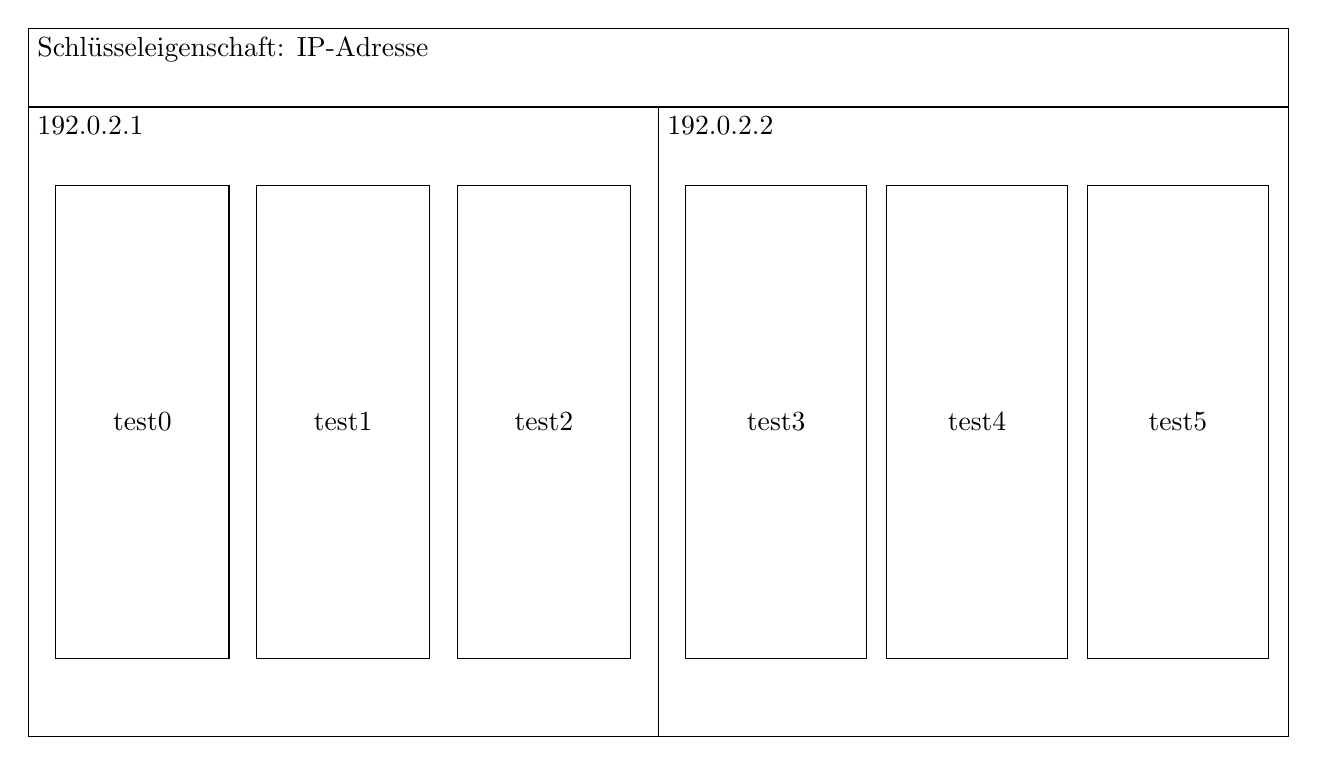
\begin{tikzpicture}
\node (rect) [rectangle, draw, minimum width=160mm, minimum height=90mm, anchor= north west] at (0,0) {};
\node [below right] at (rect.north west) {Schlüsseleigenschaft: IP-Adresse};

\node (rectA) [rectangle, draw, minimum width=80mm, minimum height=80mm, anchor= north west] at (0,-1) {};
\node [below right] at (rectA.north west) {192.0.2.1};

\node (rectA0) [rectangle, draw, minimum width=22mm, minimum height=60mm, anchor= north west] at (0.35,-2) {};
\node [] at (rectA0.center) {test0};
\node (rectA1) [rectangle, draw, minimum width=22mm, minimum height=60mm, anchor= north west] at (2.9,-2) {};
\node [] at (rectA1.center) {test1};
\node (rectA2) [rectangle, draw, minimum width=22mm, minimum height=60mm, anchor= north west] at (5.45,-2) {};
\node [] at (rectA2.center) {test2};

\node (rectB) [rectangle, draw, minimum width=80mm, minimum height=80mm, anchor= north west] at (8,-1) {};
\node [below right] at (rectB.north west) {192.0.2.2};

\node (rectB0) [rectangle, draw, minimum width=23mm, minimum height=60mm, anchor= north west] at (8.35,-2) {};
\node [] at (rectB0.center) {test3};
\node (rectB1) [rectangle, draw, minimum width=23mm, minimum height=60mm, anchor= north west] at (10.9,-2) {};
\node [] at (rectB1.center) {test4};
\node (rectB2) [rectangle, draw, minimum width=23mm, minimum height=60mm, anchor= north west] at (13.45,-2) {};
\node [] at (rectB2.center) {test5};
\end{tikzpicture}
\caption{Schematische Darstellung der Visualitionmöglichkeit der Baumstruktur}
\label{fig:schem}
\end{figure}
 
Die HTML-Seite ist in Abbildung~\ref{fig:VisualPageAll} zusehen. 
Es wird eine Baumkarte anhand der IP-Adresse erzeugt. 
Im linken Bereich des Fensters ist der Navigationsbereich zu erkennen. 
Es wird das ausgewählte Set A angezeigt, welches für die ungeschützte Datenmenge steht, Set B steht somit für die geschützte Datenmenge.
Zum wechseln zwischen den beiden Datenmengen sind zwei Schaltflächen mit den Beschreibungen A und B zu erkennen.
Unter den beiden Schaltflächen sind zwei Auswählmenüs, das obere zur Auswahl der Visualisierungsmethode, das untere zur Auswahl der Eigenschaft, welche zum erstellen der Baumkarte verwendet werden soll.
Darunter sind verschiedene Paragraphen, welche die Eigenschaften einer ausgewählten Datei wieder geben.
Die ausgewählte Datei in der Abbildung ist dataAlice1, welche in der Visualisierung im rechten Teil des Fensters als linke grüne Box zu erkennen ist.
Durch das anklicken der Box werden die Eigenschaften dieser Datei angezeigt. 
Dargestellt wird ein Beispiel nach dem in Kapitel~\ref{Kap:Szenarios} aufgeführten Beispielszenarios.
Eine genauere Beschreibung der Visualisierung im rechten Teil der Abbildung~\ref{fig:VisualPageAll} folgt im nächsten Kapitel. 

\begin{figure}[H]
\includegraphics[width=0.7\textwidth]{../pic/VisualPageAll.png}
\captionof{figure}{FileEntryVisual HTML-Seite mit Beispieldaten aus Kapitel~\ref{Kap:Szenarios}}
\label{fig:VisualPageAll}
\end{figure}

\todo{FileEntryPage beschreiben und Funktionen zeigen}

\chapter{Hauptteil} \label{Kap:Szenarios}

Um die Visualisierungen darstellen zu können werden Daten benötigt, die verschiedenen Benutzern gehören.
Diese Daten sollen wie bereits ausgeführt als geschützte Daten und ungeschützte Daten vorhanden sein. 
Dafür wird im folgenden ein Szenario definiert, anhand welchem die Visualisierungen Beispielhaft dargestellt werden. 
Dieses Beispiel ist Hypothetisch und es gibt keine zugrunde liegenden Daten. 
Die Verkehrs- und Metadaten werden für jeden Benutzer so gewählt das diese sich unterscheiden. 
Für die genauen Daten werden Standartwerte und Beispieledaten aus anderen Quellen verwendet. 

    \section{Beispiel: Alice und Bob}
Um die Visualisierungen an einem Beispiel zu erläutern wird ein Szenario definiert welches die Benutzung des Dokumentenspeichers und die verwendeten Daten definiert.
Dazu werden zwei Benutzer Alice und Bob definiert, welche sich beide in Hamburg befinden und sich in den Verkehrs- und Metadaten unterscheiden, sodass wir sie anhand dieser klar unterscheiden können.
Alice und Bob laden jeweils drei hypothetische Dateien mit und ohne die Verwendung einer Methode zum Anonymisieren ihrer Daten hoch.
Alice Dateien sind dataAlice1, dataAlice2 und dataAlice3 und Bobs Dateien sind dataBob1, dataBob2 und dataBob3 und haben alle unterschiedliche Dateigrößen.
Die Verkehrs- und Metadaten für diese Dateien sind so gewählt das sie nicht realitätsfern sind und sich eignen die verschiedenen Visualisierungen daran aufzuzeigen. 
Es wird angenommen das die Dateien von Alice und Bob einzeln in einem Abstand von mehreren Minuten hochgeladen werden.
Für die Verwendung einer Methode zum Anonymisieren ihrer Daten betrachten zwei Fälle:
\begin{enumerate}
\item Die Verwendung eines Proxys, welcher von Alice und Bob verwendet wird.
\item Die Verwendung des Tor-Netzwerks von Alice und Bob
\end{enumerate}

Für die Benutzer nehmen wir folgende Verkehrs- und Metadaten an: 
\paragraph{Alice}
\begin{itemize}
  \item IP: 
  \begin{itemize}
  \item IP-Adresse: 192.0.2.1
  \item Lat: 53.5770988464355 Lon: 10.0190000534058
  \item Land: Deutschland Region: Hamburg Stadt: Hamburg
  \end{itemize}
  \item Headerfigerprint:  
  \begin{itemize}
  \item Accept: text/html, application/xhtml+xml, application/xml;q=0.9,*/*;q=0.8
  \item Accept-Encoding: gzip, deflate
  \item User-Agent: Mozilla/5.0 (Macintosh; Intel Mac OS X 10\_11\_6) AppleWebKit/601.7.7 (KHTML, like Gecko) Version/9.1.2 Safari/601.7.7
  \end{itemize}
\end{itemize}

\paragraph{Bob}
\begin{itemize}
  \item IP: 
  \begin{itemize}
  \item IP-Adresse: 192.0.2.2
  \item Lat: 53.5830001831055 Lon: 9.98130035400391
  \item Land: Deutschland Region: Hamburg Stadt: Hamburg
  \end{itemize}
  \item Headerfigerprint:  
  \begin{itemize}
  \item Accept: text/html, application/xhtml+xml, application/xml;q=0.9,*/*;q=0.8
  \item Accept-Encoding: gzip, deflate
  \item User-Agent: Mozilla/5.0 (Windows NT 10.0; Win64; x64; rv:60.0) Gecko/20100101 Firefox/60.0
  \end{itemize}
\end{itemize}

    \subsection{IP-Adressen bezogene Visualisierung} \label{ipVis}

\todo{Die Quotes sind fucked up}
In Abbildung~\ref{fig:ungIpTM} und der Abbildung~\ref{fig:ungIpM} werden die Beispieldaten von Alice und Bob mit dem Visualisierungstool des Dokumentenspeichers dargestellt.
Die Abbildung~\ref{fig:ungIpTM} zeigt die Visualisierung der TreeMap nach dem schematischem Beispiel aus Abbildung~\ref{fig:schem}. 
In Abbildung~\ref{fig:ungIpTM} ist ein blauer Kasten zu erkennen welche den Titel: \glqq Key: ipAddress\grqq trägt und damit die Angezeigt Eigenschaft die IP-Adresse beschreibt.
In diesen Kasten sind zwei orange Kästen eingebettet.
Beide Kästen tragen einen Titel, der obere \glqq Key: 192.0.2.1\grqq, die Ip-Adresse von Alice, und der untere \glqq Key: 192.0.2.2\grqq, die IP-Adresse von Bob.
In den oberen Kasten, welcher mit Alice's IP-Adresse betitelt ist, sind 3 weitere grüne Kästen eingebettet, welche für die Dateien test0, test1 und test2 stehen.
Im unteren Kasten, welcher mit Bob's IP-Adresse betitelt ist, sind 3 rote Kästen eingebettet, welche die Dateien test3, test4 und test5 darstellen.
Die Farbe der einzelnen Kästen ist ausschlaggebend für die Ebene des Eintrags in der Baumstruktur.
Der blaue Kasten stellt den Wurzelknoten dar.
Die orangen Kästen sind die Kästen die eine verwendete IP-Adresse darstellen.
Die darunter angeordneten Kästen haben eine Farbe abhängig von der IP-Adresse welcher sie zugeordnet sind, sodass alle unter einer IP-Adresse angeordnete Dateien die selber Farbe haben, sodass ihre Zusammengehörigkeit sofort sichtbar ist.In Abbildung~\ref{fig:ungIpM} ist eine Karte von Hamburg Zentrum zu erkennen.
Auf dieser Karte sind 2 Standpunkte markiert.
Ein Punkt bei Lat: 53.5770988464355, Lon: 10.0190000534058, welcher mit dem Vorgegebenen Standpunkt von Alice übereinstimmt.
Der zweite Punkt liegt bei Lat: 53.5830001831055 Lon: 9.98130035400391, welcher dem Vorgegebenen Standpunkt von Bob entspricht.
Beim überfliegen eines Punktes mit der Maus wird für jeden Punkt die zugehörige IP-Adresse angezeigt und die Anzahl von Dateien, welche von dieser IP-Adresse hochgeladen wurden.

\begin{figure}[H]
\includegraphics[width=0.7\textwidth]{../pic/vec/IP-Proxy-SetA-tree3.PNG}
\captionof{figure}{Darstellung der ungeschützten Beispieldaten von Alice und Bob}
\label{fig:ungIpTM}
\end{figure}

\begin{figure}[H]
\includegraphics[width=0.5\textwidth , height=0.4\textheight]{../pic/IP-Proxy-SetA.PNG}
\captionof{figure}{Darstellung der ungeschützten Beispieldaten von Alice und Bob}
\label{fig:ungIpM}
\end{figure}

Die Darstellung der Daten spiegelt somit die definierten Beispieldaten korrekt wieder und erlaubt es die jeweiligen Daten den richtigen Benutzer zu zuordnen. Der Servicebetreiber sieht kennt somit die Position von Alice und Bob und kann die von ihnen Hochgeladenen Dateien an der IP-Adresse identifizieren.

Beim Betrachten des ersten Falls, der Verwendung eines Proxys erhalten wir die Visualisierung wie in Abbildung~\ref{fig:PIpTM} und Abbildung~\ref{fig:PIpM}.
In Abbildung~\ref{fig:PIpTM} ist nur ein orangener Kasten für die IP-Adresse des Proxys dargestellt.
Alle sechs definierten Dateien, test0 bis test5, sind dieser IP-Adresse zugeordnet und als grüne Kästen unter der IP-Adresse des Proxys angeordnet.
In Abbildung~\ref{fig:PIpM} ist ein Standpunkt in Berlin markiert.
Der Standpunkt liegt bei Lat: 52.5167 Lon: 13.4. 

\begin{figure}[H]
\includegraphics[width=0.7\textwidth]{../pic/IP-Proxy-SetB-tree3.PNG}
\captionof{figure}{Darstellung der Beispieldaten von Alice und Bob bei der Verwendung eines Proxys}
\label{fig:PIpTM}
\end{figure}

\begin{figure}[H]
\includegraphics[width=0.5\textwidth , height=0.2\textheight]{../pic/IP-Proxy-SetB.PNG}
\captionof{figure}{Darstellung der Beispieldaten von Alice und Bob bei der Verwendung eines Proxys}
\label{fig:PIpM}
\end{figure}

Es ist klar zu erkennen das durch die Verwendung eines Proxys in Abbildung~\ref{fig:PIpTM} und die ursprüngliche Visualisierung der ungeschützen Beispieldaten aus Abbildung~\ref{fig:ungIpTM} sich unterscheiden. 
Dies gilt auch für Abbildung~\ref{fig:ungIpM} und Abbildung~\ref{fig:PIpM}.
Ein Servicebetreiber kann anhand der IP-Adresse oder dem daraus resultierenden Standpunktes die Dateien eines Benutzer zusammen gruppieren.
In Abbildung~\ref{fig:ungIpTM} können alle Dateien der jeweiligen IP-Adresse dessen Besitzers zugeordnet werden, somit die Beispieldaten korrekt dargestellt werden.
Die Visualisierung nach Abbildung~\ref{fig:PIpTM} und Abbildung~\ref{fig:PIpM} lässt diese Zuordnung nicht mehr zu. 
Alle Dateien sind unter der IP-Adresse des Proxys angeordnet worden, somit wurde eine Anonymitätsmenge über der IP-Adresse der Proxys gebildet.
Da jede Datei der selben IP-Adresse zugeordnet ist muss ein Servicebetreiber somit annehmen das alle Dateien von dem selben Benutzer stammen.
Dies widerspricht klar den definierten Daten, welche zwei Benutzer definieren, und zeigt somit eine Erfolgreiche Anonymisierung der Daten durch die Verwendung eines Proxys im Hinblick auf die IP-Adresse.

Die entstehender Visualisierungen beim betrachten des zweiten Falls sind in Abbildung~\ref{fig:TIpTM} und Abbildung~\ref{fig:TIpM} zu sehen.
In der Abbilung~\ref{fig:TIpTM} sind sechs verschiedene orange Kästen für sechs verschiedene IP-Adressen abgebildet.
Jeder IP-Adresse sind eine Datei zugeordnet, welche als verschieden farblich Markierter Kästen der jeweiligen IP-Adresse untergeordnet wurde.
\begin{description}[style=nextline]
%\centering
\item[81.7.10.29] Datei: test0, Farbe: Grün
\item[129.13.131.140] Datei: test1, Farbe: Rot
\item[2.202.33.28] Datei: test2, Farbe: Lila
\item[81.169.133.228] Datei: test3, Farbe: Braun
\item[85.197.58.203] Datei: test4, Farbe: Pink
\item[178.63.80.54] Datei: test5, Farbe: Grau
\end{description}

Für jede dieser IP-Adressen ist in der Karte in Abbildung~\ref{fig:TIpM} ein Standort abgebildet, welche über Deutschland verteilt sind. 
\begin{description}
\item[1] Nuremberg - Lat:50.8919 Lon:11.8682
\item[2] Karlsruhe (Innenstadt-Ost) - Lat:49.0096 Lon:8.41217
\item[3] Frankfurt am Main - Lat:50.1109 Lon:8.68213
\item[4] Berlin (Charlottenburg-Wilmersdorf) - Lat:52.5239 Lon:13.3214
\item[5] Cologne - Lat:50.9872 Lon:6.89416
\item[6] Falkenstein - Lat:49.0976 Lon:12.4869
\end{description}

\begin{figure}[H]
\includegraphics[width=0.7\textwidth]{../pic/IP-Tor-SetB-tree3.PNG}
\captionof{figure}{Darstellung der Beispieldaten von Alice und Bob bei der Verwendung des Tor-Netzwerks}
\label{fig:TIpTM}
\end{figure}

\begin{figure}[H]
\includegraphics[width=0.4\textwidth]{../pic/IP-Tor-SetB.PNG}
\captionof{figure}{Darstellung der Beispieldaten von Alice und Bob bei der Verwendung des Tor-Netzwerks}
\label{fig:TIpM}
\end{figure}

Der Vergleich von Abbildung~\ref{fig:ungIpTM} und Abbildung~\ref{fig:TIpTM} zeigt einen deutlichen Unterschied der beiden Visualisierungen.
Während wie bereits ausgeführt in Abbildung~\ref{fig:ungIpTM} die Beispieldaten korrekt gruppiert visuell dargestellt werden. 
Lässt die Darstellung aus Abbildung~\ref{fig:TIpTM} und Abbildung~\ref{fig:TIpM} dies nicht mehr zu.
Da alle Dateien einer anderen IP-Adresse zugeordnet wurden muss ein Servicebetreiber annehmen das alle Dateien von einem anderem Benutzer stammen, somit 6 Benutzern, welche über Deutschland verteilt sind. 
Dies widerspricht klar den definierten Daten und zeigt eine weitere erfolgreiche Anonymisierung der Daten durch die Verwendung des Tor-Netzwerks.

Die Betrachtung der beiden Fälle zeigt verschiedene Möglichkeiten der Anonymisierung der Daten durch die Verwendung eines Proxys und des Tor-Netzwerks.
Beide Schutzmethoden haben im Hinblick auf die IP-Adresse einen derart ausreichenden Effekt gehabt, das die Visualisierungen der Beispieldaten mit und ohne die Verwendung der Schutzmethode klar erkennbare Unterschiede in der Visualisierung erzeugt haben.

    \subsection{Headerfingerprint bezogene Visualisierung}
Der Headerfingerprint wird wie im Kapitel~\ref{ipVis} beschrieben mit einer sog. TreeMap und einer dieser TreeMap zugrundeliegender Baumstruktur.
Nur die Schlüsseleigenschaft wird für diese Visualisierung von der IP-Adresse auf den Headerfingerprint geändert.
Für die ungeschützten Beispieldaten von Alice und Bob erhalten wir die Visualisierung nach Abbildung~\ref{fig:ungHTM}.
Zuerkennen sind zwei orange Kästen für die beiden verschiedenen Headerfingerprints.
Dem oberen Orangen Kasten mit dem Headerfingerprint db9080... sind drei Dateien test0, test1 und test2 zugeordnet, welche alle farblich grün markiert sind.
Dem unteren Orange n Kasten mit der Headerfingerprint 428eda... sind die drei Dateien test3, test4 unt test5 zugeordnet, welche farblich rot markiert sind.

\begin{figure}[H]
%\includegraphics[width=0.7\textwidth]{../pic/IP-Tor-SetB.png}
\includegraphics[width=0.7\textwidth]{../pic/Header-Proxy-SetA.png}
\captionof{figure}{Darstellung der Beispieldaten von Alice und Bob bei der Verwendung eines Proxy}
\label{fig:ungHTM}
\end{figure}

Wie in Abbildung~\ref{fig:ungIpTM} stellt Abbildung~\ref{fig:ungHTM} die Zusammengehörigkeit von den Dateien test0, test1 und test2 sowie den Dateien test3, test4 und test5 richtig dar.

Bei Betrachtung der Visualisierung der Beispieldaten bei der Verwendung eines Proxys erhalten wir die Visualisierung nach Abbildung~\ref{fig:PHTM}.
Diese Visualisierung ist mit der Visualisierung der ungeschützten Beispieldaten in Abbildung~\ref{fig:ungHTM} identisch. 
Der Headerfingerprint von Alice ist dargestellt sowie die Dateien von Alice test0, test1 und test2 sind diesem Headerfingerprint zugeordnet.
Der Headerfingerprint von Bob ist ebenfalls dargestellt und die Beispieldateien von Bob test3, test4 und test5 sind diesem zugeordnet.

\begin{figure}[H]
\includegraphics[width=0.7\textwidth]{../pic/Header-Proxy-SetA.png}
\captionof{figure}{Darstellung der Beispieldaten von Alice und Bob bei der Verwendung eines Proxy}
\label{fig:PHTM}
\end{figure}

Bei Betrachtung des zweiten Falls der Verwendung des Tor-Netzwerkes entspricht die Visualisierung der Abbildung~\ref{fig:THTM}.
Zu erkennen ist das ähnlich der Abbildung~\ref{fig:PIpTM} alle Dateien unter einem Headerfingerprint angeordnet sind.
Header-Tor-SetB.png
\begin{figure}[H]
\includegraphics[width=0.7\textwidth]{../pic/Header-Tor-SetB.png}
\captionof{figure}{Darstellung der Beispieldaten von Alice und Bob bei der Verwendung des Tor-Netzwerkes}
\label{fig:THTM}
\end{figure}

Die Verwendung des Tor-Netzerks hat somit zur Folge das die Dateien und Alice und Bob unter alle unter einem einzelnem Headefingerprint gruppiert werden. 
Für den Servicebetreiber bedeutet dies das anhand des Headerfingerprints die Dateien alle von einem einzelnen Benutzer stammen. 
Dies steht klar mit de definierten Beispieldaten, welche zwei benutzer Alice und Bob vorsehen im Konflikt.

Während die Verwendung eines Proxys keinen Effekt auf die verwendeten Header hatte und somit der Headerfingerprint der Benutzer trotz Benutzung des Proxys gleich geblieben ist. 
Hat die Verwendung des Tor-Netzwerks dazu geführt das die Headerfingerprints von Alice und Bob beide durch einen standardisierten Headerfingerprint ersetzt wurden und somit die Zuordnung der Dateien zu den jeweiligen Benutzern nicht mehr möglich war.

Die Verwendung des Tor-Netzwerks hat somit eine Anonymitätsmenge für die Eigenschaft des Headerfingerprints erzeugt, in welcher Menge die Dateien Anonym sind und den Benutzern Alice und Bob nicht zugeordnet werden können.


    
    \subsection{Zeit bezogene Visualisierung}
    
    
    
    \subsection{Vergleich der Schutzmethoden}
Bei Betrachtung der Verschiedenen Visualisierungen für die Darstellung des Proxys im Hinblick auf die IP-Adresse in Abbildung~\ref{fig:PIpTM} und dem Headerfingerprint in Abbildung~\ref{fig:PHTM} bietet eine Proxy, wie bereits ausgeführt, nur Schutz im Hinblick auf die IP-Adresse.
Benutzer welche einen Proxy benutzen sind somit prinzipiell über ihren Headerfingerprint zu identifizieren, falls sie keine weiteren Schutzmethoden verwenden oder ihre Headerfingerprint eindeutig genung ist um daran Identifiziert zu werden. 
Die Verwendung des Tor-Netzwerks dagegen kann wie in Abbildung~\ref{fig:TIpTM} und Abbildung~\ref{fig:THTM} gezeigt Schutz vor der Identifizierung durch die IP-Adresse und dem Headerfingerprint bieten.
Dabei ist zu beachten das die während durch die Visualisierung aus Abbildung~\ref{fig:TIpTM} ein Servicebetreiber von mehreren Benutzern ausgehen muss.
Die Visualisierung in Abbildung~\ref{fig:THTM} nur auf einen Benutzer schließe lässt.

Aus dem definierten Szenario lässt sich schließen das während die Verwendung eines Proxys und des Tor-Netzwerks im Hinblick auf die Anonymisierung der IP-Adresse gleich erfolgreich seien können, die Verwendung eines Proxys gegenüber dem Tor-Netzwerk jedoch einen deutlichen Nachteil hat bezogen auf die Möglichkeit durch seinen eigenen Individuellen Headerfingerprint identifiziert zu werden.

% Schluss
\chapter{Schluss}
\section{Zusammenfassung der Ergebnisse}
\begin{itemize}
\item Funktionalität des Dokumentenspeichers
\item Verwendungszweck des Dokumentenspeichers erfüllt?
\item Auswertung der Szenarien
\item Konklusion
\end{itemize}

\section{Limitierungen}
\begin{itemize}
\item Dokumentenspeicher sehr simple, nicht vollständig implementiert
\item Dokumentenspeicher reicht für Darstellung von einfachen Szenarien, Verwendung von echt Daten möglich, jedoch Visualisierungen passend ? Aussagekräftig ?
\item Einfache Verwendung von Headern und verschlüssleung, verbesserungsmöglichkeiten an vielen stellen.
\item Viele Annahmen sind für die Verwendung des Dokumentenspeichers getroffen
\end{itemize}

\section{Ausblick}
\begin{itemize}
\item Verbesserung der Implementierung des Dokumentenspeichers: 
    \begin{itemize}
    \item Einfachere Benutzung
    \item Ausbau der UI(HTML-Seiten) für bessere intuitive Verwendung
    \item Verwendung eines Aussagekräftigeren Verfahrung zur bestimmung des Headerfingerprint
    \item Bereitstellung von mehr Möglichkeiten zur Visualisierung, z. B. die Verwendung der TreeMap über alle Eigenschaften 
    \end{itemize}
\item Evulation der Visualisierungen im bezug auf die Angemssenheit und Aussagekräftigkeit der Visualisierung.
\end{itemize}

\end{document}
